\documentclass[11pt,a4paper]{article}
\usepackage[utf8]{inputenc}
\usepackage{amsmath}
\usepackage{amsfonts}
\usepackage{amssymb}
\usepackage{amsthm}
\usepackage{tikz}
\usepackage{graphicx}

\usepackage{algorithm}
\usepackage{algorithmic}
\usepackage{tabularx}
\usepackage{subcaption}

\usepackage[left=2cm,right=2cm,top=2cm,bottom=2cm]{geometry}
\author{Paul LANDRIER}
\title{Abstraction of computation graphs}

\newcommand{\bb}[1]{\mathbb{#1}}
\newcommand{\mcal}[1]{\mathcal{#1}}
\newcommand{\N}{\bb{N}}
\newcommand{\R}{\bb{N}}
\newcommand{\Cinf}{\mcal{C}^\infty}
\newcommand{\Ns}{near-semiring}
\newcommand{\sns}{sub-near-semiring}
\newcommand{\ovund}[3]{\overset{#1}{\underset{#2}{#3}}}

\date{}

\usetikzlibrary{shapes}

\newtheorem{theorem}{Theorem}

\newtheorem{definition}{Definition}
\newtheorem{ns}{Near-semiring}

\renewcommand{\leq}{\leqslant}

\newcolumntype{C}[1]{>{\centering\arraybackslash}p{#1}}

\begin{document}

\maketitle

\section{Introduction}

We try to abstract the notion of \textit{computation graphs}, having in mind the particular example of neural networks.

	Computation graphs are a type of graphs that represent a computation. Formally, in this work, we define a computation graph $(V,E,Fun,Op)$ as a directed acyclic graph $(V,E)$ together with a function $Fun:E \to F$ where $F$ is a set of functions $S \to S$ ($S$ is a fixed set, the same for all functions) and a function $Op:V \to Operator$ where $Operator$ is a set containing operators to aggregate several inputs in $S$. (Remark : usually in a computation graph, the functions are stored in the nodes and the edges represent a data dependency. We choose a different convention here to remain closer to provenance in graphs).
	
	For instance, if we want to compute the function $f(x)=e^{x^2}(x^2 + 2x + 2)$ using only the linear, "plus constant" and exponential functions, with $+$ and $\times$ operators, then we can model a possible computation with the computation graph :
	
	\begin{figure}[!h]
	\centering
	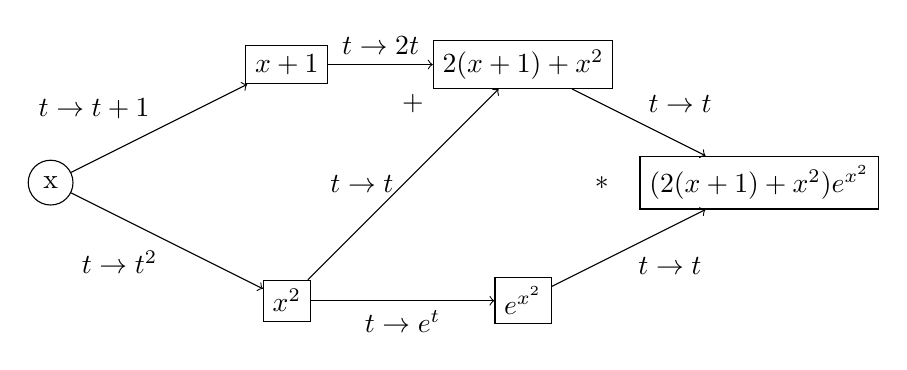
\begin{tikzpicture}
	
		\node[circle,draw] (x) at (0,0) {x};
		\node[rectangle,draw] (a) at (3,1.5) {$x+1$};
		\node[rectangle,draw] (b) at (3,-1.5) {$x^2$};
		\node[rectangle,draw] (c) at (6,1.5) {$2(x+1) + x^2$};
		\node at (4.6,1) {$+$};
		\node[rectangle,draw] (d) at (6,-1.5) {$e^{x^2}$};
		\node[rectangle,draw] (e) at (9,0) {$(2(x+1) + x^2)e^{x^2}$};
		\node at (7,0) {$*$};
		
				\path[->] (x) edge node[midway,above left] 
			{$t \to t+1$} (a);
		\path[->] (x) edge node[midway,below left]
			{$t \to t^2$} (b);
		\path[->] (a) edge node[midway,above] 
			{$t \to 2t$} (c);
			
		\path[->] (b) edge node[midway,left] 
			{$t \to t$} (c);
		\path[->] (b) edge node[midway,below] 
			{$t \to e^t$} (d);
		\path[->] (c) edge node[midway,above right]
			{$t \to t$} (e);
		\path[->] (d) edge node[midway,below right] 
			{$t \to t$} (e);
		
	\end{tikzpicture}
	\caption{One possible computation graph of $f$.}
	\label{fig:graphe_calc_ex}
	\end{figure}
	
	Let's take the example of a (non-discretized) perceptron with two inputs. If we want to model its execution using only elementary operations and the activation function $f$, we get the representation in Figure \ref{fig:perceptron}.
	
	\begin{figure}[!h]
\label{fig:graph_calc_execution}
\centering
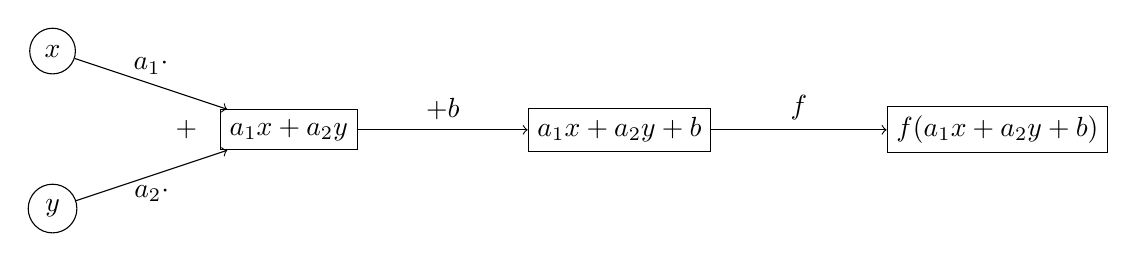
\begin{tikzpicture}

	\def\layersep{3cm}	
	
	\node[circle,draw] (x) at (0,1) {$x$};
	\node[circle,draw] (y) at (0,-1) {$y$};
	\node[rectangle,draw] (a) at (\layersep,0) {$a_1 x + a_2 y$};
	\node (plus) at (\layersep - 1.3cm,0) {+};
	\node[rectangle,draw] (c) at (2.4*\layersep,0) {$a_1 x + a_2 y + b$};
	\node[rectangle,draw] (e) at (4*\layersep,0) {$f(a_1 x + a_2 y + b)$};
	
	\path[->] (x) edge node[midway,above] {$a_1 \cdot $} (a);
	\path[->] (y) edge node[midway, below] {$a_2 \cdot$} (a);
	
	\path[->] (a) edge node[midway,above] {$ + b$} (c);
	
	\path[->] (c) edge node[midway,above] {$f$} (e);
	
	
\end{tikzpicture}
\caption{Computation graph of a perceptron.}
\label{fig:perceptron}
\end{figure}

	We could discuss another representation of perceptron with a node storing the value 1, so the $+b$ function is actually another multiplication ($\cdot b$) from this ``1-node" that enters the ($a_1 x + a_2 y$)-node. This could be convenient for the instanciation of the model we are going to developp (since it simplifies the base set of functions from ``activation-multiplication-plus constant" to ``activation-multiplication") but to model the special ``1-node" we would need to reduce the generality of the structure.

\section{Executing a computation}

\subsection{Model}

	We attempt to characterize the minimal algebraic structure required to model a computation graph. We fix $S$ the domain of the functions and, keeping in mind our targeted use case, we assume that there is only one operator : $Operator = \{ + \}$. \\

	The full computation represented by the graph cannot be expressed in a similar fashion as for provenance in graphs ($\underset{\pi \in P_{x,y}}{\sum} w(\pi)$) because composition does not distribute over $+$. In a general computation graph, the algorithm to execute the computation consists of executing the nodes following a topological ordering (by executing a node we mean executing all the functions that enters the node, sum their result and store the value).

	Another way to see it is to define the input as the nodes in the graph with in-degree 0 and the output as the node in the graph with out-degree 0. The algorithm to retrieve the function represented by the computation graph from the definition is then a recursive algorithm that builds the function starting at an output node with function identity. The ``LabelFun" attribute of input nodes is the a function that takes in argument all the inputs (let's say, as a vector) and returns the value corresponding to the particular input we are considering (typically one entry in the vector). \\

	\begin{algorithm}
	\caption{Retrieve Function}
	\label{alg:retrieve_function}
	\begin{algorithmic}[1]
	\STATE \textbf{Function} RetrieveFunction(Graph)
	\STATE \hspace{1em} Output $\leftarrow$ Graph.Output
	\STATE \hspace{1em} Result $\leftarrow$ Retrieve(Output, IdentityFunction)
	\STATE \hspace{1em} \textbf{Return} Result
	\STATE \textbf{End Function}
	\end{algorithmic}
	\end{algorithm}

	\begin{algorithm}
	\caption{Retrieve}
	\label{alg:retrieve}
	\begin{algorithmic}[1]
	\STATE \textbf{Function} Retrieve(Node, F)
	\STATE \hspace{1em} \textbf{If} Node.IsInput \textbf{Then}
	\STATE \hspace{2em} \textbf{Return} Compose(F,Node.LabelFun)
	\STATE \hspace{1em} \textbf{Else}
	\STATE \hspace{2em} Result $\leftarrow$ ZeroFunction
	\STATE \hspace{2em} \textbf{For Each} (Ancestor, G, Node) \textbf{In} Node.IncomingEdges \textbf{Do}
	\STATE \hspace{3em} Result $\leftarrow$ Result + Retrieve(Ancestor, Compose(F, G))
	\STATE \hspace{2em} \textbf{End For}
	\STATE \hspace{2em} \textbf{Return} Result
	\STATE \hspace{1em} \textbf{End If}
	\STATE \textbf{End Function}
	\end{algorithmic}
	\end{algorithm}

	\begin{figure}[!h]
	\centering
	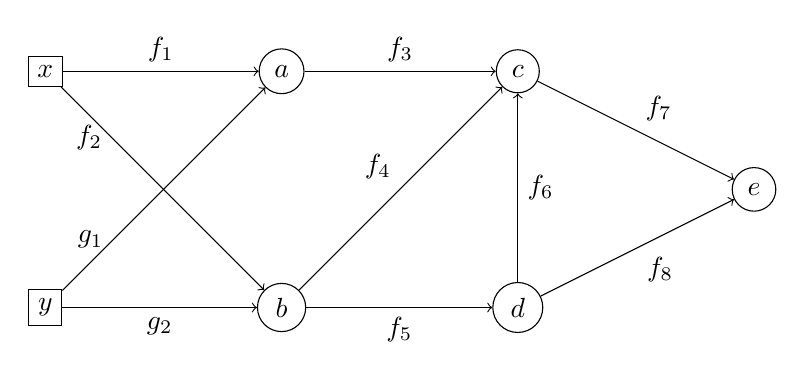
\begin{tikzpicture}
	
		\node[rectangle,draw] (x) at (0,1.5) {$x$};
		\node[rectangle,draw] (y) at (0,-1.5) {$y$};
		\node[circle,draw] (a) at (3,1.5) {$a$};
		\node[circle,draw] (b) at (3,-1.5) {$b$};
		\node[circle,draw] (c) at (6,1.5) {$c$};
		\node[circle,draw] (d) at (6,-1.5) {$d$};
		\node[circle,draw] (e) at (9,0) {$e$};
		
		\path[->] (x) edge node[midway,above] 
			{$f_1$} (a);
		\path[->] (x) edge node[near start, left=0cm]
			{$f_2$} (b);
		\path[->] (y) edge node[near start, left=0cm] 
			{$g_1$} (a);
		\path[->] (y) edge node[midway,below]
			{$g_2$} (b);
		\path[->] (a) edge node[midway,above] 
			{$f_3$} (c);
			
		\path[->] (b) edge node[midway,above left] 
			{$f_4$} (c);
		\path[->] (b) edge node[midway,below] 
			{$f_5$} (d);
		\path[->] (d) edge node [midway,right] 
			{$f_6$}(c);
		\path[->] (c) edge node[midway,above right]
			{$f_7$} (e);
		\path[->] (d) edge node[midway,below right] 
			{$f_8$} (e);
		
	\end{tikzpicture}
	\caption{An abstract computation graph.}
	\label{fig:graphe_calc_abstr}
	\end{figure}

	\paragraph{Structure needed} We consider a structure $(F,\circ,+,0,id)$. The $+$ and $\circ$ are operators $F^2 \to F$ respectively used to model aggregation and composition in the computation graph.

	Following what has been made in \textit{provenance semirings} by Green, Karvounarakis and Tannen and by Ramusat in its thesis, in order to identify the structure that best fits our application we try to identify some remarkable properties of computation graph to deduce some properties on the structure used to generalize them. We sum up the process in the table:

	\begin{figure}
		\centering
		\begin{tabular}{|C{7.5cm}|C{7.5cm}|}
			\hline 
			\textbf{Property on the computation graph} & \textbf{Algebraic traduction of the property} \\ 
			\hline 
			The edges that enter a node are not ordered & + is associative and commutative \\ 
			\hline
			The concatenation of two computation graphs is a computation graph that represent the composition of the functions & $\circ$ is associative \\ 
			\hline 
			There is a notion of zero-weight that model the fact that there is no interaction between two nodes. & There is a $0_F$ element that is a neutral element for $+$ and that is left absorbing for $\circ$. \\ 
			\hline 
			We can reuse computation previously done in a natural way. & The operator $\circ$ is right distributive over $+$. \\ 
			\hline 
			We should be able to model the identity function. & There is a neutral element $id$ for $\circ$. \\ 
			\hline 
		\end{tabular} 
	\caption{Motivation of the algebraic structure.}
	\label{fig:table_algebraic_structure}
	\end{figure}

\begin{figure}
	\centering
	\begin{subfigure}{\textwidth}
	\centering
		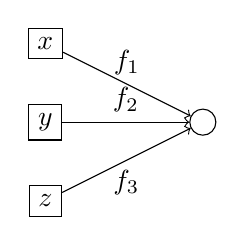
\begin{tikzpicture}
			\node[rectangle,draw] (x) at (-2.5,1) {$x$};
			\node[rectangle,draw] (y) at (-2.5,0) {$y$};
			\node[rectangle,draw] (z) at (-2.5,-1) {$z$};
			\node[circle,draw] (res) at (-0.5,0) {};
			
			\path[->,draw] (x) -- node[midway,above] {$f_1$} (res);
			\path[->,draw] (y) -- node[midway,above] {$f_2$} (res);
			\path[->,draw] (z) -- node[midway,below] {$f_3$} (res);
		\end{tikzpicture}
		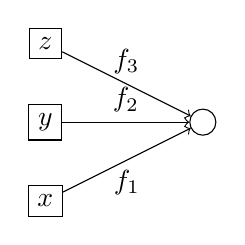
\begin{tikzpicture}
			\node[rectangle,draw] (x) at (0,-1) {$x$};
			\node[rectangle,draw] (y) at (0,0) {$y$};
			\node[rectangle,draw] (z) at (0,1) {$z$};
			\node[circle,draw] (res) at (2,0) {};
			
			\path[->,draw] (x) -- node[midway,below] {$f_1$} (res);
			\path[->,draw] (y) -- node[midway,above] {$f_2$} (res);
			\path[->,draw] (z) -- node[midway,above] {$f_3$} (res);
		\end{tikzpicture}
		\caption{A case that necessits the ``$+$" operator to be commutative and associative. Indeed, these two graphs are the same represented in two different ways, and the left one represent the element $(f_1+f_2)+f_3$ whereas the right one represents $(f_3 + f_2) + f_1$. Replacing $f_3$ by $0$ then shows that $+$ must be comutative, and using the commutativity of $+$ shows that the right expression is equal to $f_1 + (f_2 + f_3)$, so the associativity is required too.}
	\end{subfigure}

	\begin{subfigure}{\textwidth}
	\centering
		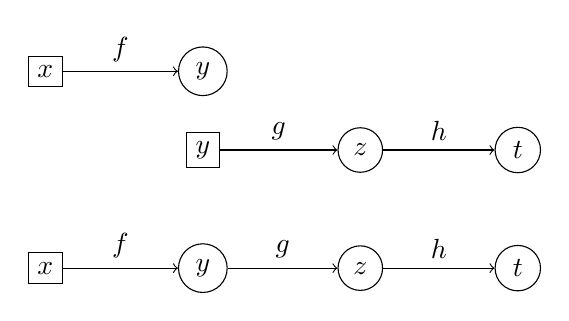
\begin{tikzpicture}
		
			\node[rectangle,draw] (x) at (0,0) {$x$};
			\node[circle,draw] (y) at (2,0) {$y$};
			\node[rectangle,draw] (y') at (2,-1) {$y$};
			\node[circle,draw] (z') at (4,-1) {$z$};
			\node[circle,draw] (t') at (6,-1) {$t$};
			
			\node[rectangle,draw] (xf) at (0,-2.5) {$x$};
			\node[circle,draw] (yf) at (2,-2.5) {$y$};
			\node[circle,draw] (zf) at (4,-2.5) {$z$};
			\node[circle,draw] (tf) at (6,-2.5) {$t$};
			
			\path[->,draw] (x) -- node[midway,above] {$f$} (y);
			\path[->,draw] (y') -- node[midway,above] {$g$} (z');
			\path[->,draw] (z') -- node[midway,above] {$h$} (t');
			
			\path[->,draw] (xf) -- node[midway,above] {$f$} (yf);
			\path[->,draw] (yf) -- node[midway,above] {$g$} (zf);
			\path[->,draw] (zf) -- node[midway,above] {$h$} (tf);
		
		\end{tikzpicture}	
		\caption{Necessity of the associativity for the modularity. The fact that the graph below, which associated element is $h\circ (g \circ f)$, represents the same element as the composition of the two graphs above, which associated element is $(h \circ g) \circ f$, is equivalent to the associativity of $\circ$. Then we can say without ambiguity that they both represent $h \circ g \circ f$.}
	\end{subfigure}

	\begin{subfigure}{\textwidth}
		\centering
		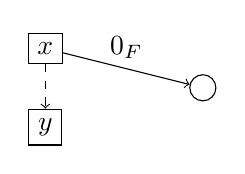
\begin{tikzpicture}
			\node[rectangle,draw] (x) at (0,0.5) {$x$};
			\node[rectangle,draw] (y) at (0,-0.5) {$y$};
			\node[circle,draw] (res) at (2,0) {};
			
			\path[->,draw] (x) -- node[midway,above] {$0_F$} (res);
			\path[->,dashed,draw] (x) -- (y);
		\end{tikzpicture}	
		\caption{Use-cases of the 0 weight. The plain arrow represent an existing edge with weight 0 (in the context of neural network for instance) and the dashed arrow represent an edge that does not exist and could be represented by the 0 element.}
	\end{subfigure}

	\begin{subfigure}{\textwidth}
		\centering
		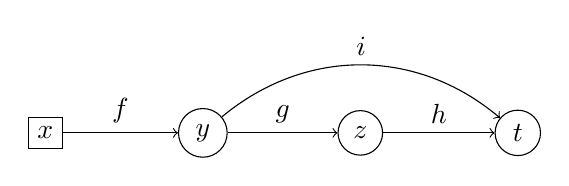
\begin{tikzpicture}
			\node[rectangle,draw] (x) at (0,0) {$x$};
			\node[circle,draw] (y) at (2,0) {$y$};
			\node[circle,draw] (z) at (4,0) {$z$};
			\node[circle,draw] (t) at (6,0) {$t$};

			\path[->,draw] (x) -- node[midway,above] {$f$} (y);
			\path[->,draw] (y) -- node[midway,above] {$g$} (z);
			\path[->,draw] (z) -- node[midway,above] {$h$} (t);
			\path[->,draw] (y) edge [bend left=40] node[midway,above] {$i$} (t);
		\end{tikzpicture}
		\caption{Illustration of the modularity allowed by the right distributivity. We can factor the expression $i~\circ~f+h~\circ~g~\circ~f$ in the smaller one $(i + g \circ h) \circ f$.}
	\end{subfigure}

	\begin{subfigure}{\textwidth}
		\centering
		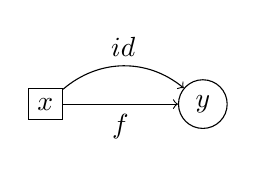
\begin{tikzpicture}
			\node[rectangle,draw] (x) at (0,0) {$x$};
			\node[circle,draw] (y) at (2,0) {$y$};
			
			\path[->,draw] (x) -- node[midway,below] {$f$} (y);
			\path[->,draw] (x) edge [bend left=40] node[midway,above] {$id$} (y);
		\end{tikzpicture}
		\caption{A use case of the identity: representing $f(x) + x$.}
	\end{subfigure}
\caption{The situations that justify the different properties discussed in Figure \ref{fig:table_algebraic_structure}.}
\label{fig:drawings_algebraic_struct}
\end{figure}

Some additional remarks on the structure:


	Since there is no natural order on incoming edges for a node, $+$ must be associative and commutative so the sum on incoming edges is well-defined. (For instance consider the node $c$ in Figure \ref{fig:graphe_calc_abstr}).

	We require the operator $\circ$ to be associative so that computations in the graph can proceed either from left to right or from right to left to retrieve the function it represents, and to ensure modularity, which allows us to define the function associated with a subgraph.

	To abstract the concept of zero-weight, we require the existence of a neutral element $0$ which is a left absorbing element for the $\circ$ operator and which is a neutral element for $+$.

	We require the left distributivity $(f+g) \circ h = f \circ h + g \circ h$ beacuse it is of theoretical interest (it is necessary for the interpretation of near-semirings as sub-near-semirings of the the complete near-semiring over a monoid), because it is a natural identity to interpret the elements as functions and because it allows for a simplification of the computation in some cases.

	Finally, we require the existence of a neutral element $id$ for $\circ$. This might not be crucial and could change, but it has interexting theoretical properties (it allows to model the one node graph for instance, which can be useful to initialize some algorithms such as Retrieve earlier). 
	\\

The axiom identified are those of a near-semiring, with two differences (+ is not assumed to be commutative in general and the ``id" does not necessarily exist). In our case, we obtain the definition:

\begin{definition}[Near-semiring]

	A \textit{near-semiring} $(F,+,\circ,0_F,id)$ is a set $F$ equiped with two binary operations $+,\circ$ and two distinguished elements $0_F,id$ such that :
	
	\begin{itemize}

		\item $(F,+,0_F)$ is a commutative monoid;

		\item $(F,\circ,id)$ is a monoid;

		\item $\forall (f,g,h) \in F^3$, $(f+g) \circ h = f \circ h + g \circ h$;

		\item $0_F$ is left absorbing for $\circ$, i.e. for all $f \in F$, $0_F \circ f = 0_F$.

	\end{itemize}

\end{definition}

Together with this definition comes the notion of morphism of near-semiring and of sub-near-semiring:

A sub-near-semiring of a near-semiring $(F,+,\circ,0,id)$ is a subset $G \subset F$ such that $0 \in G, id \in G$ and $G$ is stable by $+$ and $\circ$. If $G$ is a sub-near-semiring of $(F,+,\circ,0,id)$, then $(G,+,\circ,0,id)$ (for the restriction of operations + and $\circ$ to $G$) forms a near-semiring.

If $(F,+,\circ,0,id)$ and $(G,+',\circ ',0',id')$ are two near-semirings, then $\phi : F \to G$ is said to be a near-semiring morphism if it satisfies $\phi(0)=0',\phi(id)=id',\forall (f,g) \in F^2, \phi(f+g) = \phi(f) +' \phi(g)$ and $ \phi(f \circ g)= \phi(f) \circ' \phi(g)$. The image $\phi(F)$ is a sub-near-semiring of $G$.

\subsection{Examples}

We should now study a few examples of near-semiring.

\begin{ns}[Complete near-semiring over a monoid]
\label{ns:ns_over_a_monoid}
	Let $(M,+,0_M)$ be a monoid. We define $\mcal{F}$ the set of all functions $M \to M$. Then the tuple $(\mcal{F},+,\circ,0_F,id)$ where $0_F : x \mapsto 0_M$ is the zero function and $id : x \mapsto x$ is the identity function is a near-semiring, that we will call complete \Ns\ over $M$. A particular sub-\Ns\ of $\mcal{F}$ is the set of monoid endomorphisms of $M$ (it is even a semiring).
\end{ns}

\begin{ns}[Semirings]
\label{ns:semirings}
	Let $(S,+,\cdot,0,1)$ be a semiring. Then $(S,+,\cdot,0,1)$ is also a \Ns . Indeed, the axioms of \Ns\ are stricly more general than those of a semiring. The interpretation of semirings as sets of function together with the interpretation of $\cdot$ as a composition can be made through the structure of semimodules, which is itself a sub-\Ns\ of the complete \Ns\ over a monoid.
\end{ns}

\begin{ns}{Matrices over a semiring}

\end{ns}

\subsection{Universal object}

Given a \Ns\ $F$, we want to characterize the sub-near-semiring generated by a subset $G \subset F$. This notion makes sense for the usual reason: an intersection of sub-near-semiring is a \sns\ itself, and we note $<G>$ this \sns\ .

For this purpose we define a sequence of sets $(G_n)$ by $G_0=\{0,id\} \cup G$ and 
$$G_{n+1} = \left\{ \left. g \circ \left( \overset{k}{\underset{i=1}{\sum}} g_i \right) \right| \ k \in \N, g \in G, (g_i)_{1 \leq i \leq n} \in (G_n)^k \right\} .$$

	The claim is now that $<G> = \underset{n \in \N}{\cup} G_n$. Indeed, $G \subset G_0 \subset \underset{n \in \N}{\cup} G_n$, then we show by induction that $\forall n \in \N, G_n \subset <G>$ and finally we show that $\underset{n \in \N}{\cup} G_n$ is indeed a \sns\ of $F$.

\subsection{Generality of the complete semiring over a monoid.}

\begin{theorem}{Universal Form of Near-semirings}

	It is equivalent to be given:

	\begin{enumerate}

		\item a near-semiring $(F,+,\circ,0,id)$

		\item a commutative monoid $(M,+,0)$ together with a set of functions $M \to M$ containing $0$ and $id$ and stable by $\circ$ and $+$. (I.e. a \sns\ of the complete \Ns\ over $M$.)

	\end{enumerate}

\end{theorem}

\begin{proof}

	Firstly, we assume that we are given a monoid $(M,+,0)$ and a set of functions $M \to M$ containing $0$, $id$ and stable by $+$ and $\circ$ like in two. This precisely means that we are given a sub-near-semiring of the complete near-semiring over $(M,+,0)$, and hence a near-semiring.
	
	Secondly, if we are given a near-semiring $(F,+,\circ,0,id)$, we define for an element $f$ the function 
	$$\bar{f} : \left\{ 
	\begin{array}{c c c}
		F & \to & F \\
		g & \mapsto & f \circ g
	\end{array} \right. ,$$
	then we define the function $\phi : \left\{ 
	\begin{array}{c c c}
		F & \to & ((F,+,0) \to (F,+,0)) \\
		f & \mapsto & \bar{f}
	\end{array} \right.$. 
	
	The function $\phi$ is a morphism of near-semirings. Indeed: 
	\begin{itemize}
	
		\item $\phi(0)$ is the zero function since zero is left absorbing,
		
		\item $\phi(id)$ is the identity function because $\forall g \in F,id \circ g= g$,
		
		\item $\forall f_1,f_2 \in F^2,\ \forall g \in F,\ \phi(f_1 + f_2)(g)=(f_1 + f_2) \circ g = f_1 \circ g + f_2 \circ g = \phi(f_1)(g) + \phi (f_2)(g)$, hence $\phi(f_1+f_2)=\phi(f_1)+\phi(f_2)$
		
		\item $\forall f_1,f_2 \in F^2,\ \forall g \in F,\ \phi(f_1 \circ f_2)(g)=(f_1 \circ f_2) \circ g = f_1 \circ (f_2 \circ g) = \phi(f_1)(f_2 \circ g) = (\phi(f_1) \circ \phi(f_2))(g) $, hence $\phi(f_1 \circ f_2)=\phi(f_1) \circ \phi(f_2)$
	
	\end{itemize}
	Therefore, $\phi(F)$ is a sub-near-semiring of the complete near-semiring over the monoid $(F,+,0)$.

\end{proof}

	This theorem is interesting because it clearly indicates a direction for further investigation -if we want to instantiate the theoretical framework, we should define computation graphs over some monoids- and a limit of the expresiveness of the theory. However, it does not provide any information on the structure of near-semirings. For instance, we have an analoguous theorem on groups that states that all groups are subgroups of a bijection group, but this is of little interest when we want to study the structure of groups (like classification of finite abelian groups).


It might be interesting to note that for the example of computation graphs we restrict ourselves to finitely generated monoids, because the computation only involves a finite number of elements.

\section{Instantiation of the theory}

	\subsection{Layer-Wise Relevance Propagation}
	
		[Founded on LRP overview, https://iphome.hhi.de/samek/pdf/MonXAI19.pdf]
		
		[Dependance or not on an execution, want to do the computation once or several times]
		
	Layer-Wise Relevance Propagation (LRP) is a technique used to explain the prediction made by a neural network on one of its execution. The idea of the technique is to propagate backwards the contribution (or the \textit{relevance}) of neurons in the network to the final prediction of the model. The general formula is 
		$$ R_j = \underset{k}{\sum} \frac{z_{j,k}}{\sum_j z_{j,k}} R_k .$$
		
	The value $R_j$ is the score of the neuron $j$, and it is computed by summing over all neurons $k$ in the next layer the term $\frac{z_{j,k}}{\sum_j z_{j,k}} R_k$, where $R_k$ is the relevance of neuron $k$ and $\frac{z_{j,k}}{\sum_j z_{j,k}}$ represents the extent to which neuron $j$ contributed to the relevance of the neuron $k$.
		
	The normalization term ensures that vanishing phenomenoms cannot occur: the sum of the relevances of neurons on a given layer is preserved.
		\\
		
	We should now discuss the interpretation of LRP as an instantiation of our model.
		
	On the one hand, we can model LRP with generalized computation graphs. Indeed, the input nodes of the computation graphs are the output neurons of the network (or even the only neuron corresponding to the class predicted, since the value of other neurons is set to zero), the edges of the computation graph are the reversed edges of the neuron and the associated function is the multiplication by the scalar $\frac{z_{j,k}}{\sum_j z_{j,k}}$ (between neurons $k$ and $j$).
	
	However, on the other hand, this model might have a limited interest.
		
	\subsection{Shapley Values}
	
	Any chance it helps for Shapley values?

\section{Training a model}

Want to add a derivative $d$. Forces to add a $\cdot$. What identities ? $\to$ $d(f \circ g)$ ?

\section{Experiments ?}

\section{Further Investigations}

	Other types of NN ?

\end{document}
